\section{HAMPI: A Solver for String Constraints}
A lot of automatic analysis, testing, and verification tools can be reduced to a constraint generation phase and a constraint solving phase. The seperation of these two phases have leveraged more reliable and maintainable tools. In addition to that, increasing availability and efficiency of many off-the-shelf constraint solver makes the approach even more compelling. Hampi \cite{hampi} is designed and implemented as a constraint solver for string-manipulating programs. Hampi constraints express membership in regualar language, fixed size context-free language and membership predicates. Given a set of constraints, hampi will give the string that satisfies all the constraints or report unsatisfiable. The experiment showes that Hampi is efficient in finding SQL injections by static and dynamic ananlysis on web applications and powerful in automated bug finding in system testing of c programs.
 
Many programs, like web applications, take string as inputs, manipulate them and then use them in sensitive operations as database queries. String constraint solver plays a very important role in automatic testing\cite{pathfeasibility, database, fuzzing}, verifying the correctness of program outputs\cite{stringanalysis}, and finding security faults\cite{injection, webapp}. Writing a string constraints solver is a very time-consuming work, and integrating it will cause less maintainable system. Therefore, Hampi is designed and implemented to meet this need as a third-party module that can be easily integrated into a variety of applications.     

Hampi constraints express membership by regular language, fixed size context-free language. It may contain a fixed size string variable, context-free language definition, regular language definition and operations, and language-membership predicates. Given a set of string constraints over a string variable, Hampi outputs a string that satisfies all the constraints or reports that the constraints are unsatisfiable. Hampi is used as a component in testing, analysis, and verification applcations. Hampi can also be used to solve the intersection, containment, and equivalence problems for regular and fixed size context free languages.

A key feature for Hampi is that the fixed-sizing of regular and context free grammar. This feature differentiate Hampi with other string constraints solvers that used in many testing and analysis applications. Fixed-sizing is not a handicap for a constraint solver, but allows more expressive languages and many operations upon context-free language that would be undecidable without fixed-sizing. Fixed-sizing also renders the satisfiability problem solved by Hampi more tractable.
\begin{figure}[h]
\centering
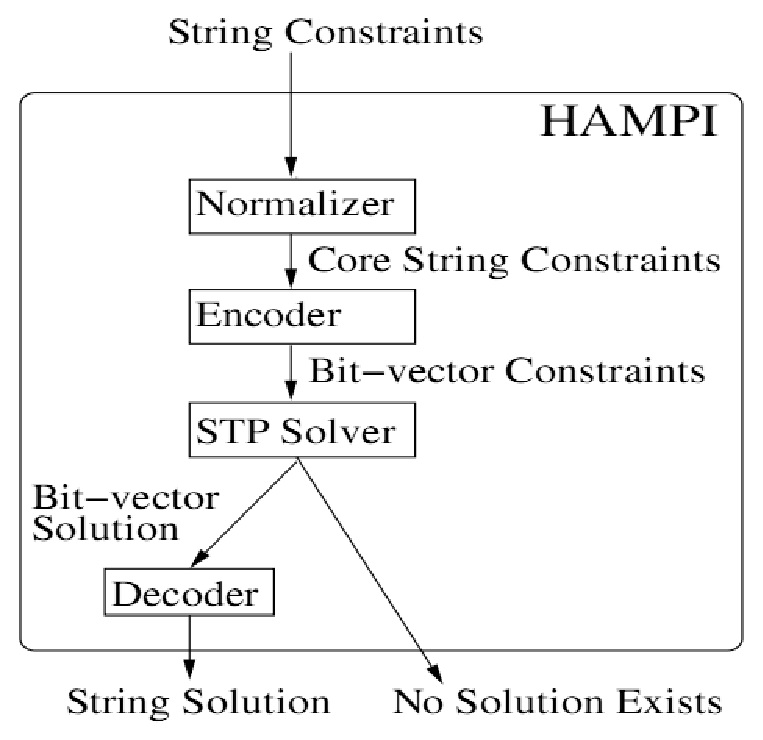
\includegraphics[scale=0.6]{hampi.eps} 
\caption{\label{fig:Hampi} Schematic view of Hampi string solver. }
\end{figure}
Hampi works in four steps as indicated in figure 1: the first is to normalize the input constraints to formal forms which are called core string constraints. The core string constraints are expressions of the form $v\in R$ or $v\notin R$, where $v$ is the input fixed-size string varible, and $R$ is the regular expression. Second, translate the core string constraints into quantifier-free logic of bit-vectors which are fixed-size, ordered lists of bits. Third, hand over the bit-vector constraints logic that Hampi uses to STP\cite{STP} which is a constraints solver for bit-vectors and arrays. Fourth, according to the report provided by STP, we get the result whether the original string constraints is satisfiable, if yes, generate a satisfying assignment in its bit-vector language and output a string solution; otherwise, report unsatisfiable. The procedure is illustrated as following graph:

We discuss the prominent feature and illustrate its language input by example. Hampi input enables the encoding of string constraint generated from the typical testing and security applications. The language supports the declaration of fixed-size variables and constraints, regular language operations, membership predicates, and the declaration of context free and regular languages, temporaries and constraints.

\begin{figure}[h]
\centering
\includegraphics[scale=0.6]{hampiinput.eps} 
\caption{\label{fig:Hampiinput} The Hampi Input Structure}
\end{figure}

Var is the string variable declared of the size specified. If all the constraints of the Hampi are satisfiable, var will be afforded value meets all the constraints. Sometimes, the application requires the constraint solver to consider all the string up to a fixed size. This end could be achieved by one of the following two ways: (1) repeatedly applying Hampi for different fixed size up to the given maximum size; (2) adjusting the constraints to allow "padding" of the variable. 

Hampi allows the standard notation Extended Backus-Naur Form(EBNF) to specify context free grammar in input. Terminals are enclosed in double quotes(e.g., "SELECT"), and productions are seperated by vertical bar symble ($|$). Grammars may contain special symbols for repetition (+ and *) and character ranges(e.g.,[a-z]).

Reg is the declaration of regular language. Regular languages are defined as following four regular expressions:(i) a singleton set with a string constant; (ii) a concatenation or union of regular languages; (iii) a repetition of a regular language; (iv) a fixed sizing of a context free language. Every regular language can be defined by the first three of these operations.  

Vals are temporary variables that act as shortcuts for expressing constraints on expressions that are concatenations of the string varibles and constants.

Assert is the key word that used by Hampi to express the membership of strings in regular languages.

After parsing all the Hampi input, Hampi normalize the string constraints into core form. The core string constraints are an internal intemediate representation that is easier to be encoded into bit-vector logic than raw Hampi input is. A core string constraints specifies membership in a regular language. A core string constraint is expressed in the form $StrExp\in RegExp or StrExp\notin RegExp$, where $StrExp$ is an expression composed of concatenations of string constants and occurrences of the string variable, and $RegExp$ is a regular expression.

The algorithm Hampi uses to create regular expressions that specify the set of strings of fixed length that are derivable from the context free grammar:
\begin{enumerate}
	\item Expand all special symbols in the grammar, like repitition, option, character range.
	\item Remove $\epsilon$ productions.
	\item Take the following steps to construct the regular expression that encodes all fixed size strings of the grammar: (i) precompute the shortest and longest size of the string that can be generated from every nonterminal(i.e. upper bound and lower bound). (ii) given a size $n$ and a nonterminal $N$, examine all the possible productions for $N$. For each $N\rightarrow S_1S_2...S_k$, where each $S_i$ could be nonterminal or terminal, enumerate all possible partitions of $n$ characters to $k$ grammar symbols. Then, create sub-expressions recursively and combine the sub-expressions together with a concatenation operator. Memoization the intermediate results makes this process scalable. 
\end{enumerate}   
The next phase of Hampi is to encode the core string constraints as fomulas in the logic of fixed-size bit-vectors. A bit-vector is fixed size, ordered list of bits. The fragment of bit vector logic that is used by Hampi contains standard boolean operations, extracting sub-vectors, and comparing bit vectors. Hampi asks STP for a satisfying assignment to the resulting bit-vector formula. If STP found one, Hampi decodes it and produce a string solution for the input constraints, otherwise Hampi will terminate and report that the string constraints is not satisfiable. The encode procedure is as follows:
\begin{enumerate}
	\item The constant string values are enforced by Hampi as relevant elements of the bit-vector variable.
	\item Hampi encodes the union operator(+) as a disjunction in the bit-vector logic.
	\item Hampi encodes the concatenation operator by enumerating all possible distributions of the characters to the sub-expressions, encoding the sub-expression recursively, and combining the sub-formulas in a conjunction.
	\item The Kleene Star will be encoded similarly to concatenation.
	\item After STP finds a solution to the bit-vector formula (if exists), Hampi decodes the solution by reading 8-bit sub-vectors as consecutive ASC2 characters.
\end{enumerate}
We will further illustrate the procedure by the following example:\\

\indent Var v:2;\\
\indent cfg $E := "()"|EE|"("E")"$;\\
\indent reg $Efixed := fixsize(E, 6)$;\\
\indent Val $q := concat("((",v,"))")$;\\
\indent assert q in Efixed;\\
\indent assert q contains $"())"$;\\

\noindent Step 1: Normalize the constraints to core form. The results after this step are:\\ 
$c_1: ((v))\in ()[()()+(())]+[()()+(())]()+([()()+(())])$\\
$c_2: ((v))\in [(+)]*())[(+)]*$\\
\noindent Step 2: Encode the core form in bit-vector logic. We will illustrate how Hampi would encode constraint $c_1$. First of all, Hampi will create a bit-vector variable $bv$ of size $48=6*8$ bits to represent the lefthand side of $c_1$. Second, the characters are translated into the ASC2 codes corresponding to them, "(" is $40$, and ")" is $41$. Then Hampi encode the lefthand side of $c_1$ as formula $L_1$, by specifying the constant value: $L_1$: $(bv[0]=40)\wedge (bv[1]=40)\wedge (bv[4]=41) \wedge (bv[5]=41)$. Byte $bv[2]$ and $bv[3]$ will be reserved for $v$, a 2-byte variable. Similarly, the right hand side of $c_1$ will be encoded as $D_{1a}\vee D_{1b}\vee D_{1c}$. The entire bit-vector logic of constraint $c_1$ after encoding would be $L_1\vee(D_{1a}\wedge D{1b}\wedge D{1c})$. The final formula that Hampi sends to STP solver is $(C_1\wedge C_2)$.\\
\noindent Step 3: STP finds a solution that satisfies the formula: $bv[0]=40, bv[1]=40, bv[2]=41, bv[3]=40, bv[4]=41, bv[5]=41$. In the decoded ASC2, the solution is $"(()())"$(quote mark is not part of the solution string).
\noindent Step 4: Hampi reads the assignment for variable $v$ off of the STP solution, by decoding the elements of $dv$ that corresponds to $v$, i.e., element 2 and 3. It reports the solutions for $v$ as $")("$.( even though there may be other solutions possible, STP can only find one.)

The performance of Hampi is evaluated through automatic finding of SQL injection attack strings by running a dynamic analysis tool on PHP web applications. Results show that Hampi has successfully replaced Ardilla\cite{}'s custom attack generator, it solves the associated constraints quickly, finds all of the solution of $N\leq 6$, and solved all of the constraints in less than 10 seconds per constraint. 